\documentclass{article}
\usepackage[utf8]{inputenc}

\title{Reply to Editor and Reviewers}
\author{}
\date{\today}

\usepackage[style=authoryear,giveninits=true,uniquename=init]{biblatex}
% Make parenthical citations the default
\renewcommand\cite{\parencite}
%\addbibresource{sample_bibliography.bib}
\addbibresource{appendix.bib}
\addbibresource{sn-bibliography.bib}

%\usepackage{mwe}
%\usepackage{blindtext}
\usepackage{booktabs}
\usepackage{tabularx}  % in preamble

\usepackage{enumitem}
 
\usepackage{graphicx}
\usepackage{caption} % to get nicer top captions with tables
\usepackage{subcaption}

\newcommand{\mAP}{\textrm{mAP}}
\newcommand{\mysubsection}[1]{\subparagraph{#1}}

% to change the colour of text
\usepackage{xcolor}
% to strike through text
\usepackage[normalem]{ulem}
% to frame text
\usepackage{framed}

% to help with quoting added material in the revised paper 
\usepackage{quoting}
% \newcommand{\say}[1]{%
% \begin{quoting}
% #1
% \end{quoting}
% }

\newcommand{\sayold}[1]{%
{\color{olive}#1}
}



\newcommand{\saydel}[1]{%
{\color{darkgray}\sout{#1}}}

\newcommand{\saymod}[1]{%
  \texorpdfstring{\textcolor{blue}{#1}}{#1}%
}

% \newcommand{\saymod}[1]{#1}


\newcommand{\sayintro}[1]{%
  \texorpdfstring{\textcolor{olive}{#1}}{#1}%
}

\newcommand{\saynew}[1]{%
{\color{orange}#1}}

\newcommand{\reviewcomment}[3]{%
\vspace{4mm}
\textbf{C[$R_{#1}C_{#2}$]:} {\it #3}
\vspace{2mm}
}

\newcommand{\response}[1]{%
{\textbf{R:}} {#1}
}

% Change the default figure/table numbering to avoid confusion with main manuscript
\renewcommand{\figurename}{Fig.}
\renewcommand{\thefigure}{L\arabic{figure}}
\renewcommand{\thetable}{L\arabic{table}} 
\newcommand{\figref}[1]{\figurename~\ref{#1}}
\newcommand{\tabref}[1]{\tablename~\ref{#1}}
\newcommand{\subresponse}[1]{\underline{\MakeUppercase{#1}}}
% \newcommand{\enclose}[1]{\par\indent """  #1   \indent """\par}

\newcommand{\enclose}[1]{%
%    \smallskip
%    \par
%    \noindent%
%    \fbox{%
%        \begin{minipage}{\dimexpr\linewidth-2\fboxsep-2\fboxrule\relax}#1 
%        \end{minipage}%
%    }%
%    \par
\begin{framed}
#1
\end{framed}
}

\usepackage[pdfusetitle,hidelinks]{hyperref}

\begin{document}

\maketitle

In the revised document that we join with this reply, the deleted old parts are in \saydel{striked out dark gray}, the modified parts in \saymod{blue}
and the added parts in \saynew{orange}.
%
Changes made to the revised manuscript and reproduced in this letter for ease of use are highlighted using a simple frame as:
\enclose{Text from revised document.}


%%%
\section{Manuscript Modifications}

\vspace{4mm}
\textbf{C[$MR_{1}$]:} {\it
The paper introduces triplet segmentation, a new task that grounds surgical action triplets ⟨instrument, verb, target⟩ directly at the instance level. To support this, the authors build CholecTriplet-Seg, an extension of the CholecTriplet dataset that links each triplet to its corresponding instrument mask following a clear annotation protocol. They also present TargetFusionNet, a Mask-2Former based model with a target-aware fusion module aimed at improving the (still challenging) target prediction component. Across recognition, detection, and segmentation, the method consistently outperforms adapted baselines. Both the dataset and code are made publically available.

All three reviewers (R2, R5, R6) provide overall positive evaluations and recommend acceptance. They agree that the work is novel, well motivated, and fills a clear gap by introducing triplet segmentation and releasing a valuable dataset to support it.

Positive points across reviewers:
\begin{itemize}[noitemsep,nolistsep]
\item Novel task and dataset (R2, R5, R6): All reviewers highlight the contribution of CholecTriplet-Seg and the relevance of grounding triplets at the instance level.
\item Methodological soundness (R2, R5, R6): TargetFusionNet is viewed as well motivated, and results show consistent improvements over baselines.
\item Good presentation and reproducibility (R2, R5, R6): The paper is clearly written, code/data are public, and experiments are thorough.
\end{itemize}

Common weaknesses:
\begin{itemize}[noitemsep,nolistsep]
\item Limited analysis of target prediction failures (R2, R6): The weakest component remains under-discussed.
\item Missing ablations and backbone analysis (R2, R5): Reviewers request clarity on how much improvement stems from the architecture vs. pretrained features such as EndoViT.
\item Single-rater annotation without inter-rater assessment (R6): Given the ambiguity of linking actions to specific instances, this is seen as a limitation.
\item Limited analysis of class imbalance and rare triplets (R2).
\end{itemize}
\vspace{2mm}
}

\vspace{4mm}
\textbf{C[$MR_{2}$]:} {\it
The paper introduces triplet segmentation, a novel task that unifies instance-level instrument segmentation with action understanding (instrument–verb–target triplets) in surgical videos. It presents CholecTriplet-Seg, an extended, densely annotated version of the Cholec80 dataset, including segmentation masks aligned with verb–target annotations, enabling pixel-level triplet grounding.

Major Strengths:
%Major Weaknesses:
\begin{enumerate}[noitemsep,nolistsep]
\item Introduces a well-motivated, novel task (triplet segmentation) bridging spatial grounding and action understanding.
\item Releases CholecTriplet-Seg: a large-scale, transparently annotated benchmark with segmentation masks linked to triplet labels.
\item Proposes TargetFusionNet with a clear design rationale (target-centric fusion) and demonstrates consistent improvements.
\item Evaluation is thorough: includes ablations, statistical significance tests, qualitative results, and adapted metrics.
\end{enumerate}

Major weaknesses:
\begin{enumerate}[noitemsep,nolistsep]
\item Target prediction performance is low ($mAP_T \approx 21-23\%$) and lacks in-depth analysis of causes (e.g., class imbalance, ambiguity, annotation noise).
\item Insufficient investigation of data imbalance across 100 triplet combinations and its impact on learning rare cases.
\item Architecture contribution is ambiguous: reviewers note that performance gains may stem more from EndoViT pretraining than the proposed fusion design; a direct EndoViT-Triplet baseline is missing, clouding attribution of improvement.
\end{enumerate}

Methodological gaps:
\begin{enumerate}[noitemsep,nolistsep]
\item No multi-rater validation for segmentation annotations (reliability concern).
\item Limited discussion of failure modes and instrument–target linking mechanism (e.g., why linking helps).
\item Missing related work on symbolic triplet grounding in surgery.
\end{enumerate}
\vspace{2mm}
}

\vspace{2mm}
\noindent\textbf{Response to Meta-Reviewers.} 
We sincerely thank the meta-reviewers for their constructive and thoughtful comments, and for recognising the novelty and relevance of triplet segmentation and the CholecTriplet-Seg benchmark. We also thank all reviewers for their detailed feedback and positive assessment. We have revised the manuscript accordingly and provide detailed, point-by-point responses below.
\vspace{2mm}

The main modifications performed to revise our manuscript address the following points:
\begin{enumerate}
    \item \textbf{Clarification and analysis of target prediction limitations.} 
    We expanded the discussion to better analyse why anatomical target prediction remains the primary bottleneck in triplet segmentation. In particular, we discuss the inherent visual ambiguity of surgical anatomy, poorly defined and inconsistent boundaries, and the impact of long-tailed target and triplet distributions. We also clarify the role of weak anatomical priors in TargetFusionNet and their limitations in resolving fine-grained semantic ambiguity. In addition, we introduced a structured failure mode analysis to improve interpretability and transparency (answers to \hyperref[reviewer_4_1]{$R_{4}C_{1}$}, \hyperref[reviewer_4_3]{$R_{4}C_{3}$}).

    \item \textbf{Dataset statistics, class imbalance, and annotation trade-offs.}
    We strengthened the presentation of dataset statistics and class frequency distributions by improving signposting in the main manuscript and adding a dedicated appendix analysis of triplet frequency versus performance. This analysis explicitly examines the effect of long-tailed supervision on rare triplet learning. We also clarify the single-rater annotation setup as a design trade-off arising from the alignment of existing datasets, and make the discussion of expected annotation ambiguity and quality control procedures more explicit (answers to \hyperref[reviewer_4_2]{$R_{4}C_{2}$} , \hyperref[reviewer_6_1]{$R_{6}C_{1}$}).

    \item \textbf{Clarifying architectural contributions versus pretrained features.}
    We clarified the respective roles of EndoViT and the proposed TargetFusionNet architecture by strengthening the methodological description and interpretation of existing ablation studies. In particular, we emphasise that EndoViT is used as a fixed source of weak anatomical priors rather than as a pretrained backbone for triplet segmentation, and that the observed performance gains arise from the proposed target-aware fusion design. We also improved signposting of architectural ablations, including early fusion, late fusion, and fusion-depth variants (answers to \hyperref[reviewer_4_4]{$R_{4}C_{4}$}, \hyperref[reviewer_5_1]{$R_{5}C_{1}$}).

    \item \textbf{Expanded related work and interpretation of instrument-triplet linking.}
    We extended the Related Work section to include prior approaches that symbolically associate action triplets with instrument actors, and clarified how triplet segmentation differs by providing explicit instance-level spatial grounding. Additionally, we include a discussion of why instance-level instrument linking improves performance (answers to \hyperref[reviewer_6_2]{$R_{6}C_{2}$}, \hyperref[reviewer_6_3]{$R_{6}C_{3}$}).
\end{enumerate}


\section{Detailed Answer to Reviewer 4}

\reviewcomment{4}{0}{
The paper introduces triplet segmentation, a new task that grounds surgical action triplets ⟨instrument, verb, target⟩ at the pixel level. It releases CholecTriplet-Seg, a dataset of ~31k annotated frames that link instance masks with action and target labels. The authors propose TargetFusionNet, which builds on Mask2Former and adds weak anatomical priors to improve target prediction. Experiments show consistent improvements across recognition, detection, and segmentation, making it the new benchmark for fine-grained surgical scene understanding.

Major strengths of the paper as a bulleted list:
\begin{itemize}[noitemsep,nolistsep]
 \item Addresses a clear gap by introducing triplet segmentation, unifying instance-level spatial grounding with action understanding in surgical videos
 \item provides a valuable benchmark with a large amount of frames linking instrument masks to verb-target annotations
\end{itemize}
}

\textbf{Response.}
We sincerely thank the reviewer for the positive summary and for highlighting the motivation and novelty of triplet segmentation, the value of the CholecTriplet-Seg benchmark, and the consistent improvements achieved by TargetFusionNet across recognition, detection, and segmentation. We further strengthened the revised manuscript with additional analysis and clarifications (see responses to C[$R_{4}C_{1}$]-C[$R_{4}C_{4}$]).



\reviewcomment{4}{1}{\phantomsection\label{reviewer_4_1}
Target prediction remains a bottleneck (mAP\textsubscript{T} only $\sim$21--23\%), and the discussion of why so is missing.}

\textbf{Response.}
We agree with the reviewer that target prediction remains the most challenging component of triplet segmentation and that the original manuscript and appendix can be improved by providing a clearer analysis of the underlying reasons.

In the revised manuscript, we add a concise clarification in the discussion explaining that anatomical targets are intrinsically harder to predict than instruments due to high visual similarity and ambiguous boundaries, which contributes to the lower target $\mAP$.

We also provide a better failure mode analysis in the appendix (see  C[$R_{4}C_{3}$]), including representative examples of target confusion. The following text has been added to the Discussion section of the manuscript:

\enclose{
Second, target segmentation still remains a bottleneck, as low target $\mAP$ directly constrains overall triplet accuracy.
\saynew{Target prediction is intrinsically harder than instrument/verb prediction due to high visual similarity and ambiguous boundaries between anatomical structures, which contributes to the lower target $\mAP$. A more detailed breakdown of failure patterns with  representative examples is provided in the appendix.}
}



%---

\begin{figure}[t!]
    \centering
    % %--- Top: Triplet Frequency %---
    \begin{subfigure}{\textwidth}
        \centering
        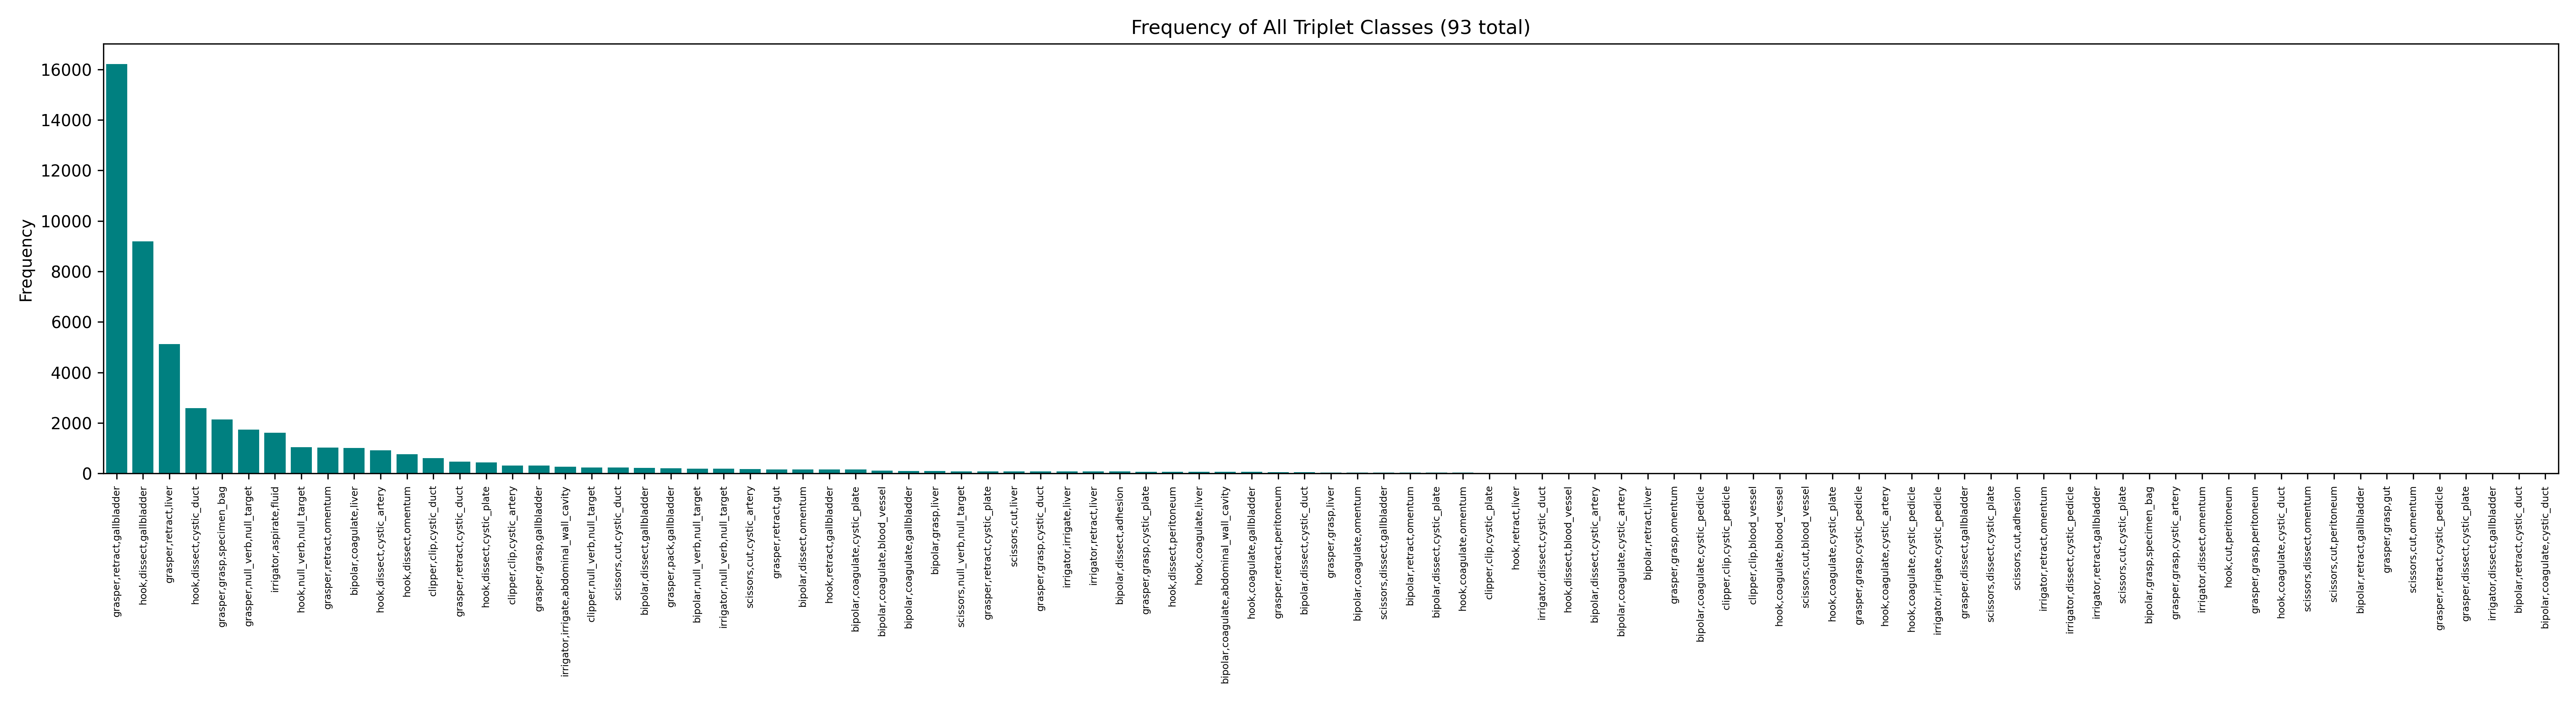
\includegraphics[width=\textwidth]{appendix_images/all_triplets_frequency.png}
        \caption{Frequency of all triplet classes.}
        \label{fig:triplet-freq}
    \end{subfigure}

    \vspace{1em}

    % %--- Bottom Row: Instrument, Verb, Target %---
    \begin{subfigure}{0.32\textwidth}
        \centering
        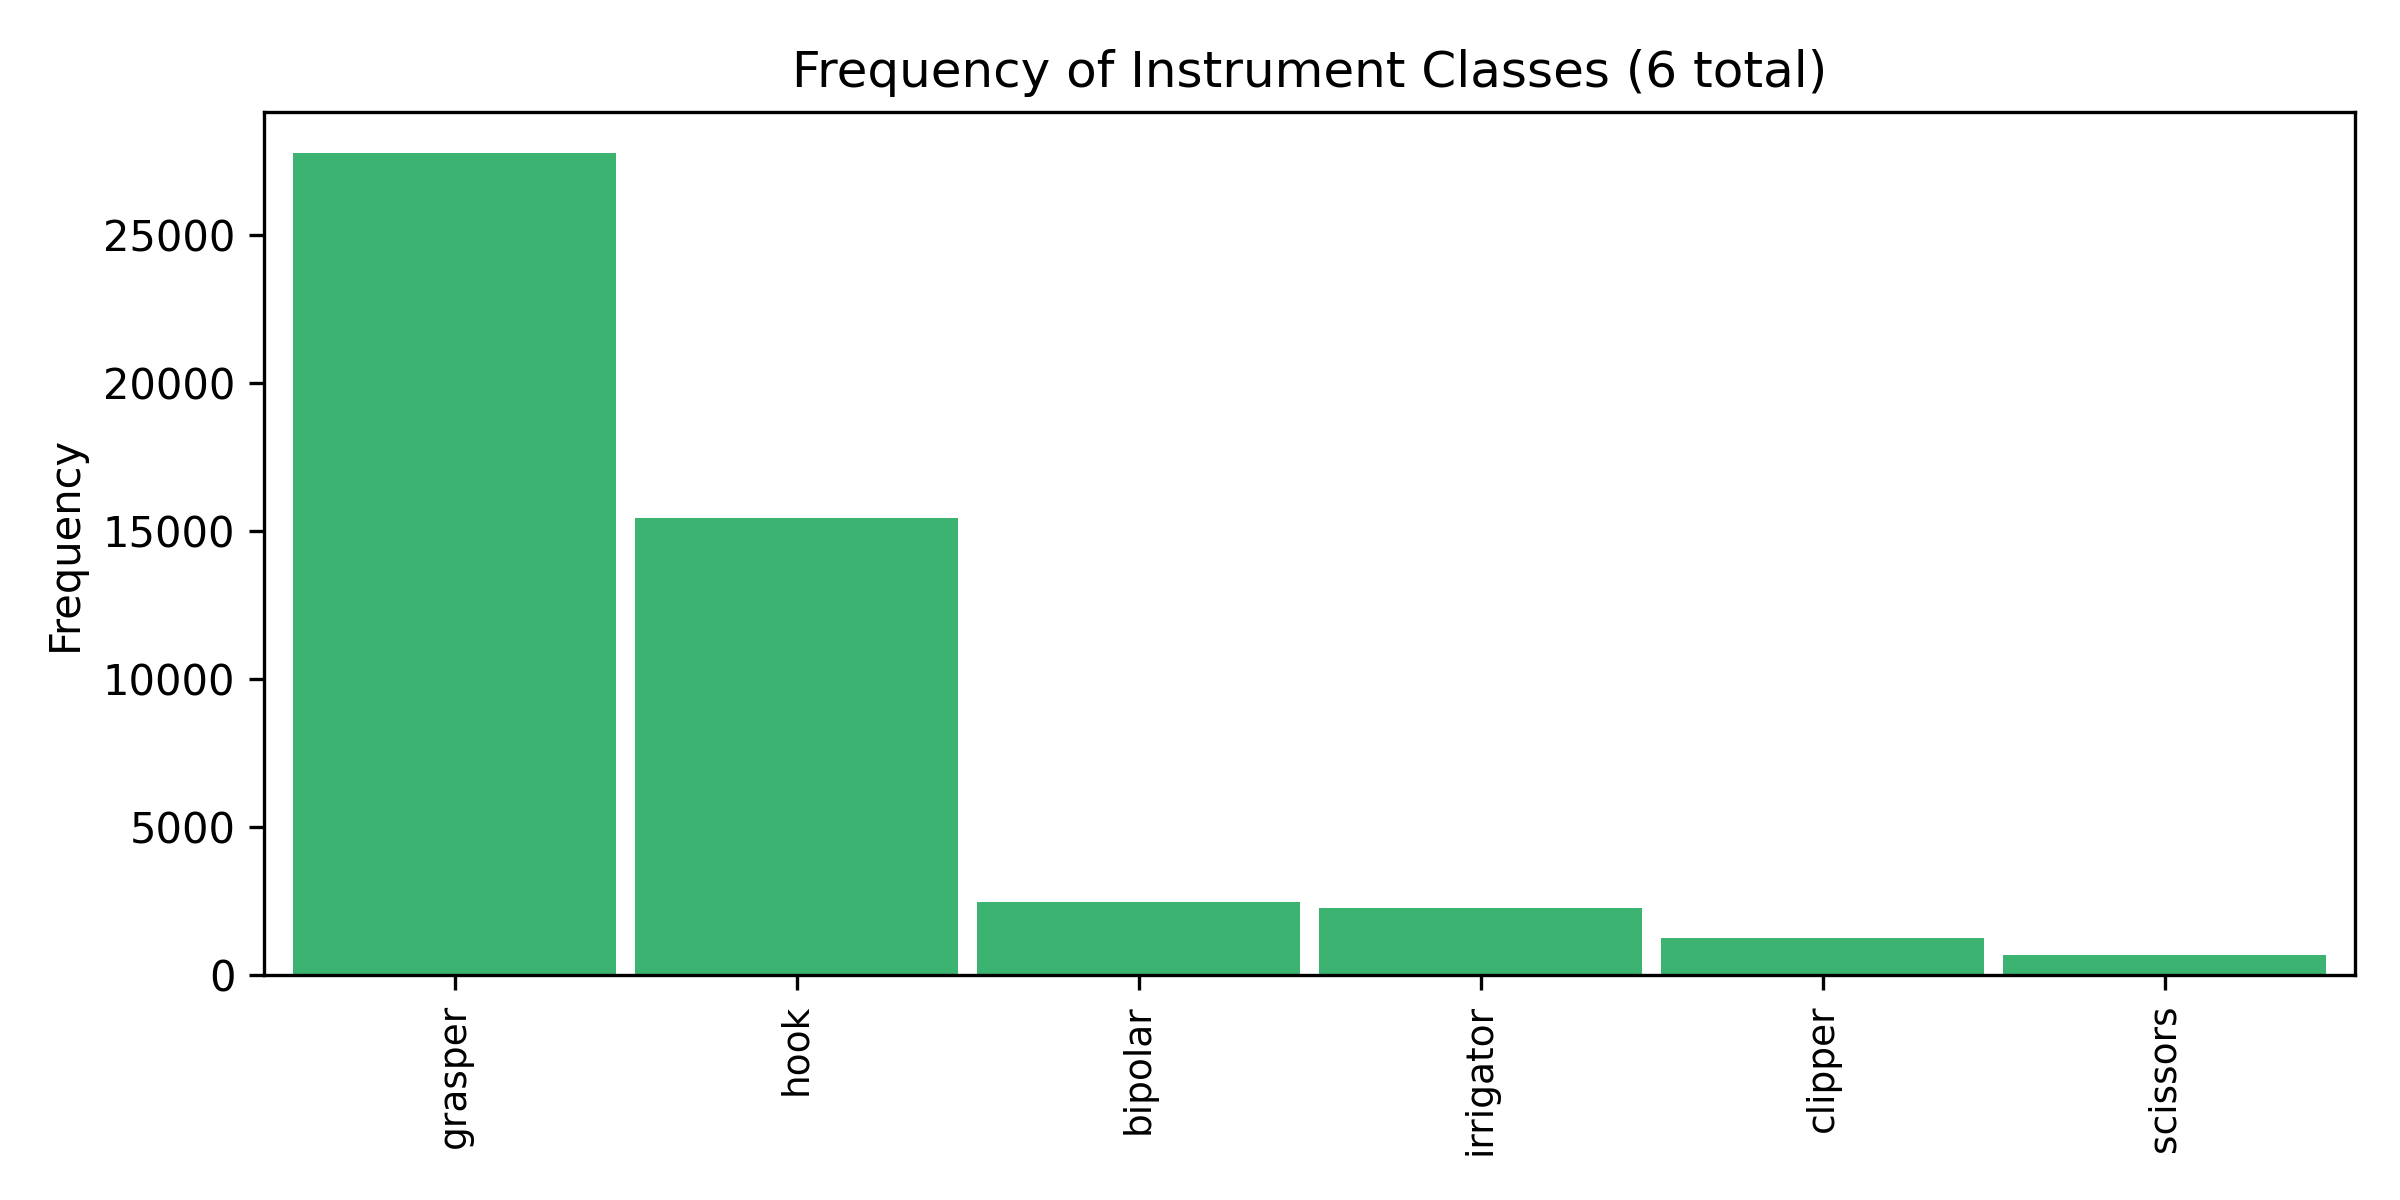
\includegraphics[width=\textwidth]{appendix_images/instrument_frequencies.png}
        \caption{Instrument frequencies.}
        \label{fig:instrument-freq}
    \end{subfigure}
    \hfill
    \begin{subfigure}{0.32\textwidth}
        \centering
        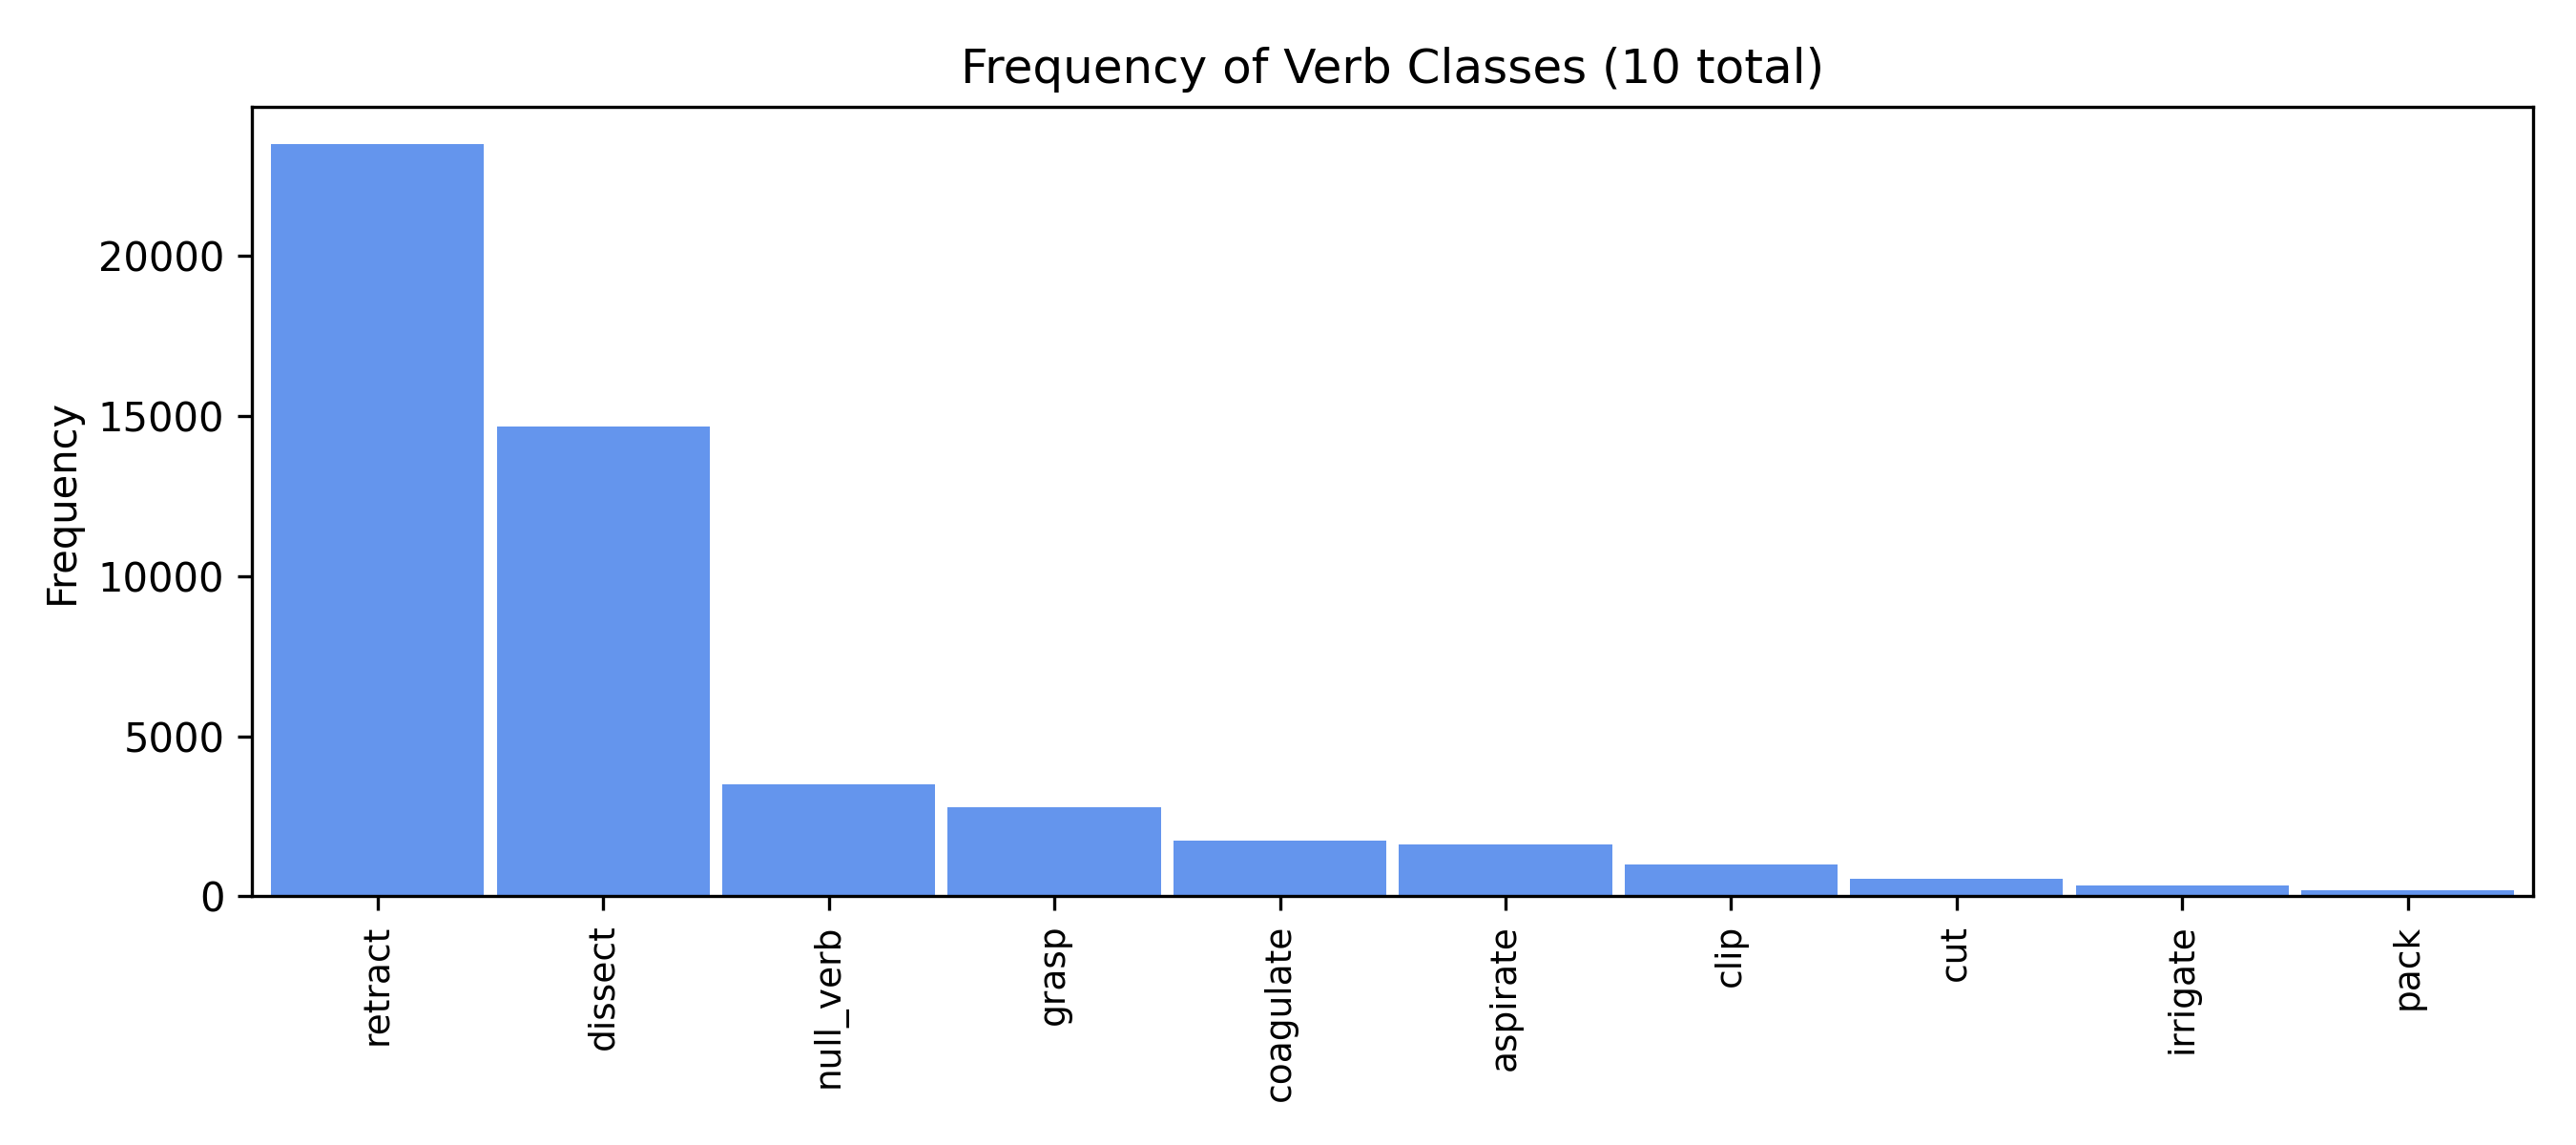
\includegraphics[width=\textwidth]{appendix_images/verb_frequencies.png}
        \caption{Verb  frequencies.}
        \label{fig:verb-freq}
    \end{subfigure}
    \hfill
    \begin{subfigure}{0.32\textwidth}
        \centering
        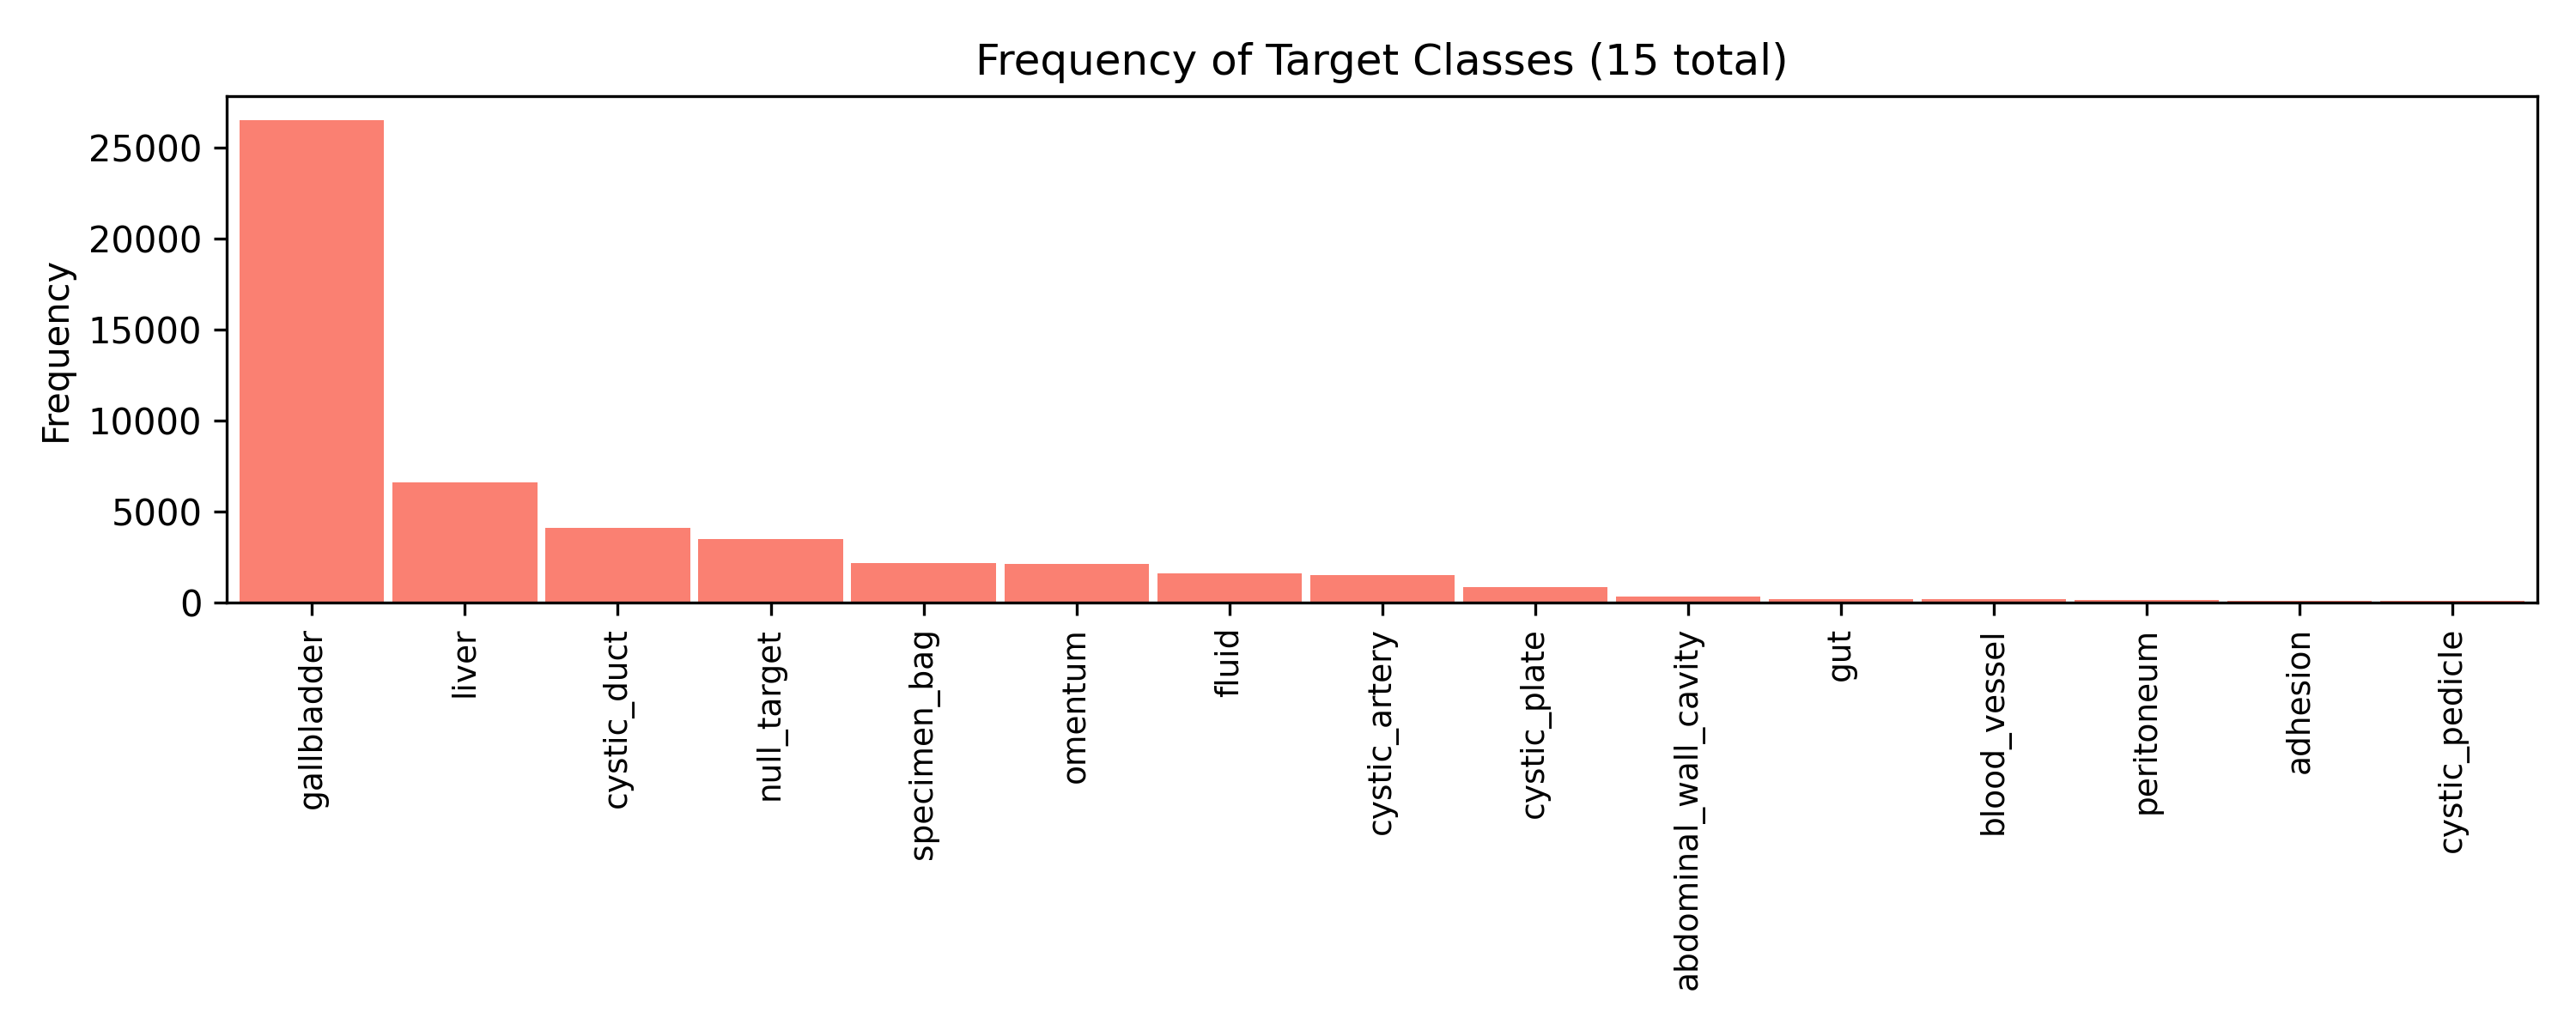
\includegraphics[width=\textwidth]{appendix_images/target_frequencies.png}
        \caption{Target  frequencies.}
        \label{fig:target-freq}
    \end{subfigure}

    \caption{Class frequency distributions in the dataset. The top row shows the frequency of all triplet classes (instrument, verb, target combinations), while the bottom row shows the distribution across individual instruments, verbs, and targets.}
    \label{fig:dataset-class-distributions}
\end{figure}


\reviewcomment{4}{2}{\phantomsection\label{reviewer_4_2}
Insufficient analysis of data distribution and potential class imbalance across the 100 valid triplet combinations. lacks discussion of how imbalance affects evaluation and whether rare triplets are learned effectively.}

\textbf{Response.}
%We thank the reviewer for this comment. 
While frequency statistics for instruments, verbs, targets, and triplets were previously reported in the appendix, we agree that the impact of class imbalance on model performance was not sufficiently analysed or discussed in the original manuscript. We also acknowledge that the appendix analysis was not clearly signposted in the main text.

In the revised version, we explicitly analyse the long-tailed distribution of valid triplet combinations and its effect on triplet segmentation performance. Triplet classes are grouped into frequent, medium-frequency, and rare categories based on their occurrence in the training set, and performance is reported separately for each group. This analysis reveals a clear degradation in performance for rarer triplets, reflecting the combined effects of limited supervision and increased semantic ambiguity.

To improve clarity without overloading the main manuscript, we now (i) explicitly highlight the long-tailed nature of the dataset in the dataset description, and (ii) provide a detailed quantitative analysis of class imbalance in a new appendix section.


Specifically, we added the following statement to the dataset description to make the class imbalance explicit and to signpost the appendix analysis:


\enclose{
The final dataset contains 30{,}955 annotated frames and 49{,}866 spatially grounded triplets from 50 cholecystectomy videos, including 15 fully annotated and 35 sparsely sampled cases (1 in 30 frames).
\saynew{
The resulting triplet dataset exhibits a strongly long-tailed distribution (see appendix).
}
}

We currently have a section and figure highlighting dataset imbalance in the appendix, which we reproduce here for clarity.

\enclose{
\paragraph{Class distribution.} The dataset exhibits a highly imbalanced (long-tailed) distribution, as shown in \figref{fig:dataset-class-distributions} [numbering altered for consistency in the response letter]. A few frequent triplets dominate the dataset, while many others occur only sparsely. This pattern is mirrored in the individual instrument, verb, and target class distributions.
}

Finally, we added a new appendix section and associated table (reproduced as \tabref{tab:triplet_frequency_analysis} in this letter) that provides a quantitative analysis of the effect of the long-tailed triplet distribution on model performance:

\enclose{
\section{\texorpdfstring{\saynew{Effect of Long-Tailed Triplet Distribution on Model Performance}}{Effect of Long-Tailed Triplet Distribution on Model Performance}}

\saynew{
CholecTriplet-Seg exhibits a long-tailed distribution over clinically valid triplet combinations, with a small number of frequent triplets accounting for a large proportion of annotations and many triplets occurring only sparsely (\figref{fig:dataset-class-distributions}). To analyse the effect of this imbalance on triplet segmentation performance, we group triplet classes into three frequency categories based on their occurrence in the training set.
}

\saynew{
Specifically, triplet classes are categorised as \textit{frequent} if they occur more than \textbf{1000} times in the dataset, \textit{medium-frequency} if they occur between \textbf{100} and \textbf{1000} times, and \textit{rare} if they occur fewer than \textbf{100} times in the training set. These thresholds are chosen heuristically to reflect the highly skewed class distribution and to enable a coarse analysis of performance trends under long-tailed supervision, rather than to define strict or optimal class boundaries.
}

\saynew{
For each frequency group, we report the average triplet segmentation performance ($mAP^{seg}_{IVT}$), summarised in \tabref{tab:triplet_frequency_analysis}. As expected, performance decreases with decreasing triplet frequency due to limited supervision and increased semantic ambiguity. 
}

}

\begin{table}[t]
\centering
\caption{\saynew{Triplet segmentation performance grouped by triplet frequency. Triplet classes are partitioned into frequent, medium-frequency, and rare groups based on their occurrence in the training set. Performance is reported using triplet segmentation mAP ($mAP_{seg}^{IVT}$).}}
\label{tab:triplet_frequency_analysis}

\small
\setlength{\tabcolsep}{4pt}
\renewcommand{\arraystretch}{1.15}

\begin{tabular}{
>{\raggedright\arraybackslash}p{0.34\textwidth}
>{\centering\arraybackslash}p{0.16\textwidth}
>{\centering\arraybackslash}p{0.24\textwidth}
>{\centering\arraybackslash}p{0.20\textwidth}
}
\toprule
\textbf{Triplet Frequency Group} & \textbf{No Triplet Classes} & \textbf{Avg. Samples / Class} & \textbf{$mAP_{seg}^{IVT}$} \\
\midrule
Frequent & 10 & 4168.9 & 0.4148 \\
Medium-frequency & 21 & 307.9 & 0.2071 \\
Rare & 62 & 24.9 & 0.04 \\
\bottomrule
\end{tabular}
\end{table}




%---

\reviewcomment{4}{3}{\phantomsection\label{reviewer_4_3}
Limited discussion of failure modes beyond video.}

\textbf{Response.}
We 
%thank the reviewer for this suggestion and 
agree that a more structured discussion of failure modes would strengthen the manuscript. To address this, we extend the failure mode analysis by systematically categorising common error patterns observed across the test set. To preserve the conciseness of the main manuscript, we place the detailed analysis in the appendix and signpost it from the main text.

In particular, the revised manuscript discusses failure modes arising from (i) missing or incorrect instrument masks, (ii) errors on rare triplet classes, (iii) confusion between visually similar targets, and (iv) action ambiguity. This structured analysis complements the previously provided qualitative video examples by offering a clearer interpretation of the dominant sources of error.

The following summary has been added to the discussion section:

\enclose{
\saynew{A more detailed breakdown of failure patterns with representative examples is provided in the appendix.}
}


A new appendix section (\saynew{Failure Mode Analysis}) has been added together with an associated figure (reproduced as \figref{fig:failure_modes} in this letter). The new appendix reads.

\begin{figure}[t!]
    \centering
    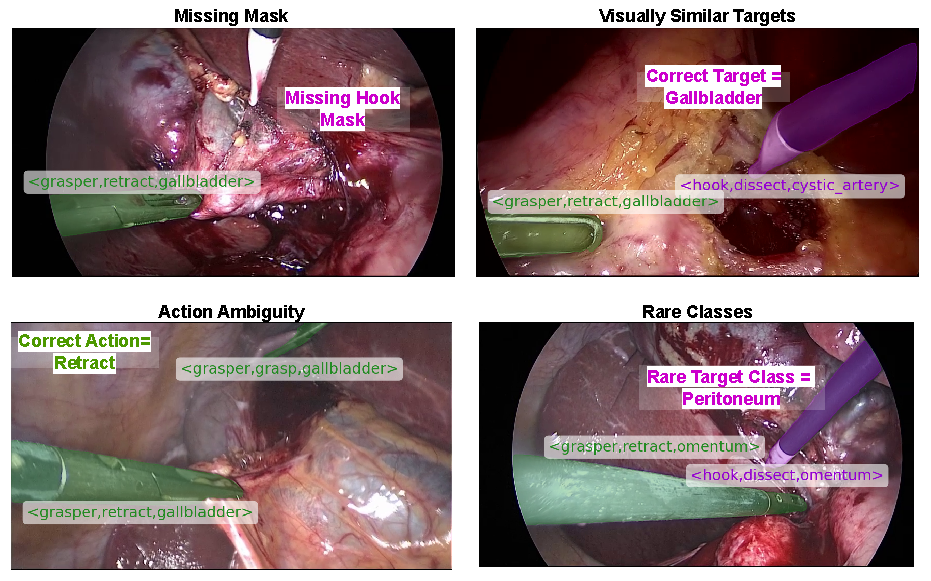
\includegraphics[width=\linewidth]{appendix_images/failure_modes.pdf}
    \caption{\saynew{
Representative failure cases in triplet segmentation.
\textbf{Top left:} missing hook instrument mask leading to incorrect triplet prediction.
\textbf{Top right:} confusion between boundaries of visually similar anatomical targets (gallbladder vs.\ cystic artery).
\textbf{Bottom left:} action ambiguity between visually similar verbs (grasp vs.\ retract).
\textbf{Bottom right:} rare target class (peritoneum) with limited training examples.
}}
    \label{fig:failure_modes}
\end{figure}

\enclose{

\section*{\saynew{Failure Mode Analysis}}

\saynew{
To better understand the remaining errors in triplet segmentation, we analyse common failure patterns observed across the test set. Rather than isolated prediction noise, these errors consistently arise from a small number of recurring scenarios, which we categorise below.
}

\saynew{
\textbf{Missing or incorrect instrument masks.}
Instance-level triplet segmentation depends on accurate instrument instance prediction. We observe occasional missing, fragmented, or incorrectly assigned instrument masks, which result in incorrect triplet predictions. Joint optimisation for triplet segmentation can slightly degrade raw instance mask quality compared to training instance segmentation in isolation, reflecting a trade-off between instance precision and higher-level semantic reasoning.
}

\saynew{
\textbf{Rare class errors.}
Classes with very low training frequency are more likely to be misclassified due to limited supervision. This effect is particularly pronounced for infrequent anatomical targets such as the peritoneum.
}

\saynew{
\textbf{Visually similar targets}
Anatomically adjacent or visually similar structures (e.g., cystic artery, cystic duct, cystic pedicle, and gallbladder) are occasionally confused, especially when boundaries are ambiguous and weakly defined. While weak anatomical priors provide coarse spatial context, they do not always resolve fine-grained semantic distinctions between such targets.
}

\saynew{
\textbf{Action ambiguity}
Some surgical actions exhibit subtle visual differences (e.g., grasp vs. retract), making them difficult to distinguish from single frames without explicit temporal context. As a result, verb misclassification can occur even when the instrument instance and anatomical target are correctly localised.
}

\saynew{
Representative examples of these failure modes are shown in \figref{fig:failure_modes}, illustrating typical errors arising from missing masks, rare target classes, visually similar anatomical structures, and action ambiguity.
These failure modes highlight intrinsic challenges of fine-grained laparoscopic scene understanding and motivate future work on improved instance segmentation, anatomical modelling, better metrics, and temporal reasoning.
}



}


%---

\reviewcomment{4}{4}{\phantomsection\label{reviewer_4_4}
Ablating the segmentation architecture would strengthen claims about the contribution of target-aware fusion.}

\textbf{Response.}
%We thank the reviewer for this suggestion. 
We would like to clarify that architectural ablations were already conducted to isolate the contribution of the proposed target-aware fusion mechanism.
%
In particular, the comparison between Mask2Former-Triplet and TargetFusionNet represents an explicit architectural ablation in which the target-aware fusion module is removed entirely, while keeping the backbone, decoder structure, and training protocol unchanged. This comparison isolates the effect of introducing target-aware fusion.

In addition, the manuscript already reports ablations evaluating alternative fusion strategies (early and late fusion), multitask loss formulations, and fusion-depth variants that vary the number of decoder layers where fusion is applied. These experiments are described in the ablation section and appendix.

In the revised manuscript, we improve clarity by explicitly stating that Mask2Former-Triplet serves as an architectural ablation that removes the target-aware fusion module. Specifically, we add the following clarification in the Baselines section:


\enclose{
Mask2Former-Triplet: extends Mask2Former with a 100-class triplet head that jointly predicts instance masks and triplet labels, removing heuristic matching and providing a strong baseline for comparison with TargetFusionNet. \saynew{This model serves as an explicit architectural ablation, removing the target-aware fusion module while keeping the backbone, decoder structure, and training protocol unchanged.
}
}

%%%
\section{Detailed Answer to Reviewer 5}

\reviewcomment{5}{0}{
The paper aligns a semantic segmentation dataset and a surgical action triplet dataset to create a new benchmark called triplet segmentation. It also proposes a new model architecture to attempt the task and benchmarks it against comparable methods.

Major strengths of the paper as a bulleted list:
\begin{itemize}[noitemsep,nolistsep]
 \item The major strength of this paper is that the proposed task of triplet segmentation is a logical and meaningful evolution of the existing popular triplet recognition task. The dataset and methods used here appear suitable for establishing this task as a new benchmark in the SDS community. The dataset has a decent size and the task and metric seem well defined. The code and data are openly available.
 \item The design of the proposed method TargetFusionNet is well motivated (focus on target recognition). The evaluation is thorough, including qualitative results and significance tests. The benchmark methods are mostly well chosen, considering that the task is new and no prior methods for this exact task exist.
 \end{itemize}

[...]

The authors make a meaningful contribution in proposing a new benchmarking task and providing a dataset and methodology for it. The evaluation is generally sound, with the unfortunate omission of ablating the impact of large-scale pretraining.
}

\textbf{Response.}
We thank the reviewer for the positive comments and for recognising the value of triplet segmentation as a meaningful evolution of triplet recognition, together with the contribution of releasing a well-defined benchmark with openly available code and data. We also thank the reviewer for the encouraging feedback on TargetFusionNet and the experimental evaluation. We address the remaining concerns in the comments below (see response to C[$R_{5}C_{1}$]).


\reviewcomment{5}{1}{\phantomsection\label{reviewer_5_1}
Considering that the EndoViT features improve the performance of TargetFusionNet, it would be interesting to see a pretrained EndoViT finetuned for triplet segmentation to create an EndoViT-Triplet method as another benchmark (analogous to Mask2Former-Triplet). Without clarity on how much the architecture vs.\ EndoViT pretraining contributes, the value of the TargetFusionNet architecture remains somewhat unclear.}

\textbf{Response.}
We thank the reviewer for this thoughtful comment and for highlighting the importance of disentangling the contributions of large-scale pretraining and architectural design.
%
We would like to clarify that EndoViT is not used as a pretrained backbone or representation extractor for triplet segmentation in our method. Instead, EndoViT is employed as a fixed source of anatomical priors that provide coarse regional cues. These priors are derived from a tissue segmentation task with a different (albeit related) label space (CholecSeg8k with different class names) and are not fine-tuned on CholecTriplet-Seg. Their role is therefore not to improve visual representation learning, but to inject auxiliary spatial context that helps disambiguate instrument–target interactions.

TargetFusionNet is specifically designed to fuse these weak priors with instance-level queries in a controlled manner via gated cross-attention. The architectural contribution lies in how such priors are selectively integrated, rather than in leveraging stronger pretrained visual features. This is further supported by our ablation studies comparing TargetFusionNet to Mask2Former-Triplet (which removes the fusion module entirely) as well as early and late-fusion variants, demonstrating that the gains arise from the proposed fusion mechanism rather than increased model capacity or backbone changes.

We agree that benchmarking alternative large-scale pretrained backbones or fine-tuned EndoViT variants for triplet segmentation would be an interesting and complementary research direction. However, such experiments would address a different question, the impact of representation learning in encoders for triplet segmentation, whereas our focus in this work is on architectural inductive bias for target disambiguation under weak supervision. We now clarify this distinction explicitly in the manuscript.

The following clarification has been added to the methods section:

\enclose{
We incorporate coarse anatomical cues using inference logits from EndoViT~\cite{batic2024endovit}, trained on CholecSeg8k \cite{hong2020cholecseg8k} for tissue segmentation in cholecystectomy surgeries. EndoViT predicts six broad tissue classes that only partially overlap with the 15 anatomical target categories in our triplets, introducing class mismatches and noisy predictions. Nevertheless, these logits capture useful spatial context, such as rough anatomical boundaries (e.g., distinguishing liver regions from the gallbladder). We treat them as noisy priors rather than ground truth and integrate them into TargetFusionNet to guide target prediction.
\saynew{EndoViT is not used as a pretrained backbone but as source of weak anatomical priors, providing coarse regional cues rather than enhanced visual features. }

}

\section{Detailed Answer to Reviewer 6}

\reviewcomment{6}{0}{
The authors aim to improve supervised surgical action triplet recognition performance by spatially linking triplets to the visible instruments inside each frame. To achieve this, they introduce an extension of the CholecTriplet dataset with linked instrument instance segmentations called CholecTriplet-Seg to train and evaluate models on triplet recognition, detection and segmentation tasks. They show that a novel TargetFusionNet model outperforms baseline models in all tasks.

Major strengths of the paper as a bulleted list:
\begin{itemize}[noitemsep,nolistsep]
 \item a new enhanced version of the CholecTriplet dataset (CholecTriplet-Seg) with an extensive annotation protocol for transparency and reproducibility
 \item adapted metrics for evaluation of the new proposed triplet segmentation task
 \item a new model for triplet segmentation with improved performance in all presented tasks
\end{itemize}

[...]

The authors present a meaningful extension of the CholecTriplet dataset by linking action triplets to specific instrument instances, enabling triplet segmentation of instruments. The annotation protocol is well documented, and the resulting CholecTriplet-Seg dataset is a valuable contribution. The authors further propose TargetFusionNet, which outperforms baseline models across all considered tasks.
The work is overall well motivated and experimentally sound.
}

\textbf{Response.}
We thank the reviewer for the encouraging assessment and for highlighting the contributions of CholecTriplet-Seg, the adapted evaluation metrics for triplet segmentation, and the strong performance of TargetFusionNet across tasks. We address the detailed comments in C[$R_{6}C_{1}$]-C[$R_{6}C_{3}$].

\reviewcomment{6}{1}{ \phantomsection\label{reviewer_6_1}
No multi-rater annotation or review process for the CholecTriplet-Seg.

[...]

%However, first the dataset relies on single-rater annotations without multi-rater assessment. 
Given the ambiguity of linking triplets to specific instrument instances, even a brief discussion of expected annotation inconsistency in the main manuscript would improve the transparency of the dataset. 
}

\textbf{Response.}
We agree with the reviewer that linking action triplets to specific instrument instances can be ambiguous in certain cases, and that a multi-rater annotation process would be preferable.

CholecTriplet-Seg was constructed by aligning and extending two previously established datasets, CholecInstanceSeg and CholecT50, whose annotation protocols were already fixed. As a result, the scope for introducing additional independent annotations was limited to consistency checking and correction of clear errors. A single trained annotator therefore performed the triplet-to-instrument linkage following a detailed and explicit protocol, with multiple rounds of manual verification to ensure internal coherence.

Additional corrections were applied only in cases of clear disagreement between the source datasets, as documented in the appendix.

This limitation was already acknowledged in the original manuscript and discussed as part of the dataset design trade-offs. In the revised version, we improve clarity by making this discussion more explicit in the main dataset description and by more clearly signposting the detailed analysis already provided in the appendix.

\enclose{
Two rounds of visual inspection confirmed annotation quality, with additional statistics, details, and \saynew{discussion of design trade-offs and expected sources of annotation ambiguity} provided in the appendix.
}


\reviewcomment{6}{2}{\phantomsection\label{reviewer_6_2}
Missing prior works symbolically linking triplets to visible instruments and missing discussion about differentiation.

[...]

%Second, a 
[A]
prior method where action triplets were symbolically linked with instrument instances in the form of “actor” labels
%(DOI: 10.1007/s00464-024-10958-w) 
\cite{younis2024surgical}
should be taken into account when introducing the spatial association. Please clarify how the proposed dataset and approach differ from this prior work and why another annotation protocol was created. 
}

% \textbf{Response.}
% We thank the reviewer for pointing out related work on symbolic actor-based triplet representations. Due to the strict word limit, we prioritised improvements to the core manuscript and discussion of methods focused on the progression of spatial grounding in triplet understanding, which is the primary focus of this work.

\textbf{Response.}
We thank the reviewer for pointing out related work that symbolically links action triplets to instrument actors using an explicit actor label (DOI: 10.1007/s00464-024-10958-w), which we had previously omitted. We now explicitly cite and discuss this work in the revised manuscript.

We clarify that this prior work associates action triplets with abstract instrument roles or actors to enable responsibility attribution, without providing pixel-level localisation or instance segmentation. In contrast, our work focuses on spatial grounding at the instance level by linking each action triplet to a specific instrument mask. These approaches therefore address different levels of abstraction: symbolic responsibility assignment versus explicit spatial grounding.

We have added this work to the related work section and clarified this distinction.


\enclose{
\saynew{\cite{younis2024surgical} explored symbolic extensions of surgical action triplets by introducing explicit actor labels for responsibility attribution. However, this formulation does not provide pixel-level instance grounding of actions in the image.
}
}

\reviewcomment{6}{3}{\phantomsection\label{reviewer_6_3}
Missing discussion investigating why instrument linking improved results.

[...]

%Third, the
[The]
manuscript provides little analysis of why improvements occur with TargetFusionNet. A short discussion of possible mechanisms (e.g. reduced ambiguity or better localization cues?) would enhance the interpretation of results.
}

\textbf{Response.}
We agree with the reviewer that a brief discussion of why instance-level instrument linking improves performance would strengthen the manuscript. In the revised version, we add a concise explanation highlighting that linking actions to specific instrument instances reduces ambiguity in multi-instrument scenes and enforces spatial consistency between predicted actions and their visual evidence.
%
%The following statement has been added to the manuscript:
%
\enclose{
Our experiments demonstrate that models trained with strong instrument supervision achieve the best overall balance across instrument, verb, and target predictions, significantly outperforming weakly supervised approaches such as RDV-Det.
\saynew{Instance-level instrument linking improves performance by reducing action ambiguity in multi-instrument scenes and enforcing spatial consistency between predicted actions and their visual evidence.}
}



\printbibliography

\end{document}
